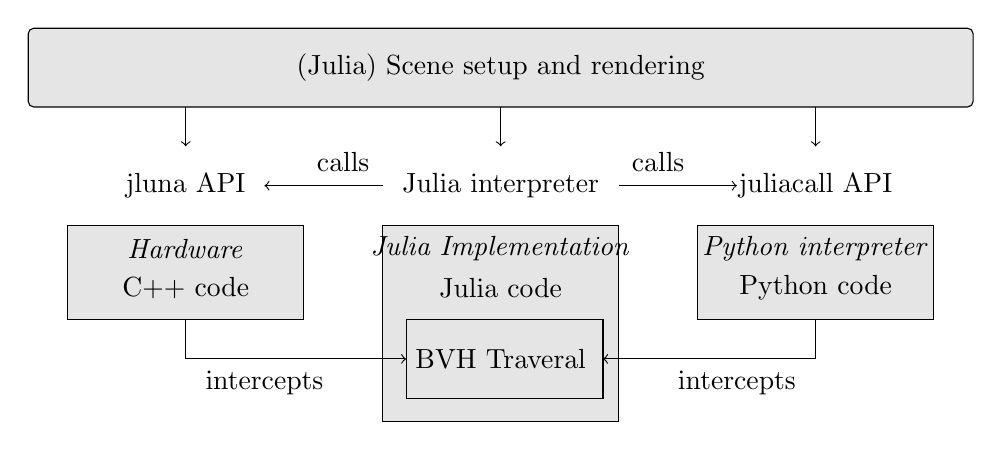
\begin{tikzpicture}

  \draw[rounded corners=2pt, fill=black!10] (0,0) rectangle (12,1);
  \node at (6,0.5) {(Julia) Scene setup and rendering};

  \draw[->] (2,0) -- (2,-.5);
  \node at (2,-1) {jluna API};

  \draw[fill=black!10] (.5,-1.5) rectangle (3.5,-2.7);

  \node at (2,-1.8) {\textit{Hardware}};
  \node at (2, -2.3) {C++ code};
  
  \draw[fill=black!10] (4.5,-1.5) rectangle (7.5,-4);
  \node at (6,-1.8) {\textit{Julia Implementation}};
  \node at (6, -2.3) {Julia code};

  \draw[fill=black!10] (4.8,-2.7) rectangle (7.3,-3.7);
  \node at (6,-3.2) {BVH Traveral};
  

  \draw[->] (2,-2.7) -- (2,-3.2) -- (4.8,-3.2);

  \node at (3,-3.5) {intercepts};


  \draw[->] (10,0) -- (10,-.5);
  \node at (10,-1) {juliacall API};

  \draw[fill=black!10] (8.5,-1.5) rectangle (11.5,-2.7);

  \node at (10,-1.8) {\textit{Python interpreter}};
  \node at (10, -2.3) {Python code};
  

  \draw[->] (10,-2.7) -- (10,-3.2) -- (7.3,-3.2);

  \node at (9,-3.5) {intercepts};


  \draw[->] (6,0) -- (6, -.5);
  \node at (6,-1) {Julia interpreter};

  \draw[->] (4.5,-1) -- (3, -1);
  \node at (4,-.7) {calls};


  \draw[->] (7.5,-1) -- (9, -1);
  \node at (8,-.7) {calls};
\end{tikzpicture}
